\section{Sistemas de Recomendação implementados}


\subsection{Sistemas baseados em filtros colaborativos}

Nestes sistemas foram utilizadas as várias avaliações dos utilizadores para se fazerem recomendações. 

\subsubsection{Filtros colaborativos baseados em utilizadores}\hfill

Neste caso, as classificações fornecidas por utilizadores com os mesmos gostos de A são usadas para fazer recomendações para A.
O método que realiza este filtro chama-se \textit{colab\_filtering()}, de seguida apresenta-se o método e explica-se o seu funcionamento.

\begin{figure}[H]
\centering
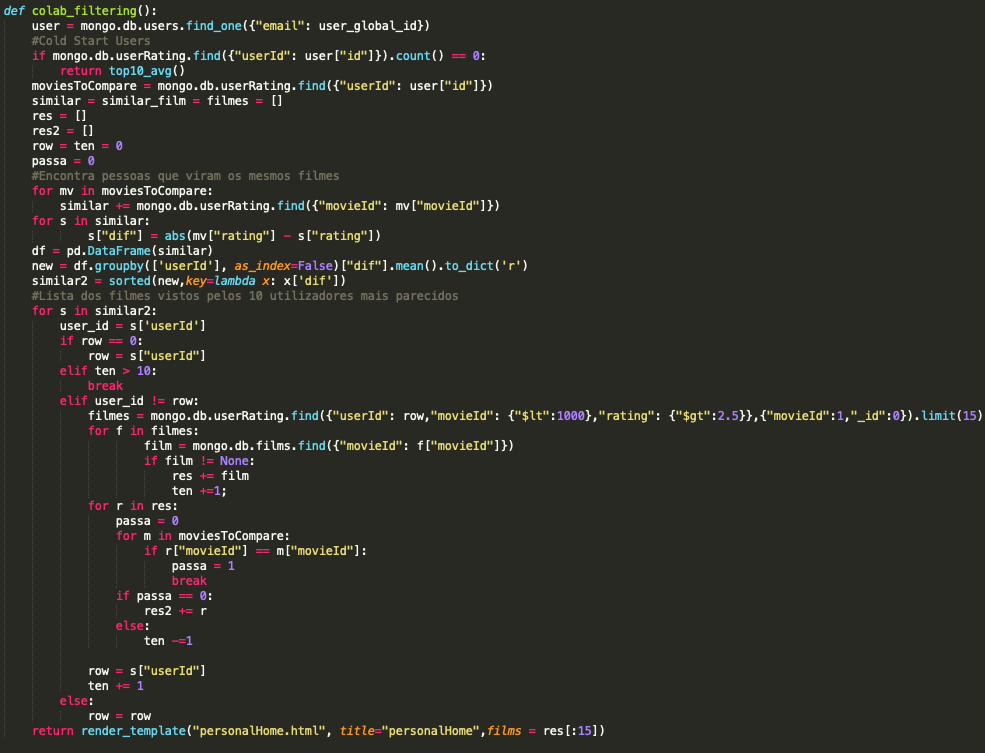
\includegraphics[width=\textwidth]{colab.png}
\caption {Função colaborative\_filtering()}
\label {fig01}
\end{figure}

Neste método, a primeira coisa a fazer é recolher os documentos com as avaliações do utilizador aos filmes por ele vistos. Nesta fase o utilizador pode não ter visto filmes ainda e solicitar o filtro colaborativo, neste caso esta função retorna-lhe os filmes mais bem cotados pelo IMDB (que têm mais chances de ser do intresse do utilizador).
\par Caso o utilizador já tenha visto um ou mais filmes estes são recolhidos e são procurados na base de dados documentos de outros utilizadores que tenham visto os mesmos filmes,sendo estes guardados num array. De seguida este array é percorrido e é calculada a diferença entre as avaliações de cada utilizador e o nosso alvo, guardando-as numa coluna extra.
Após este processo é calculada a média das diferenças por utilizador e o array resultante com duas posições (id utilizador, diferença) é ordenado por ordem crescente de diferença.
Por fim basta procurar quais os filmes avaliados por cada utilizador, percorrendo o array de utilizadores semelhantes, dos quais estes gostaram tendo o cuidado de não inserir filmes repetidos ou que o alvo já tenha visto.

\subsection{Sistemas baseados em conteúdo}

Nestes sistemas, as avaliações do utilizador, assim como os géneros dos filmes de que ele gosta, são combinados para fazer as recomendações.
O método para realizar esta abordagem chama-se \textit{filmWatchBased()}, de seguida apresenta-se o método e explica-se o seu funcionamento.

\begin{figure}[H]
\centering
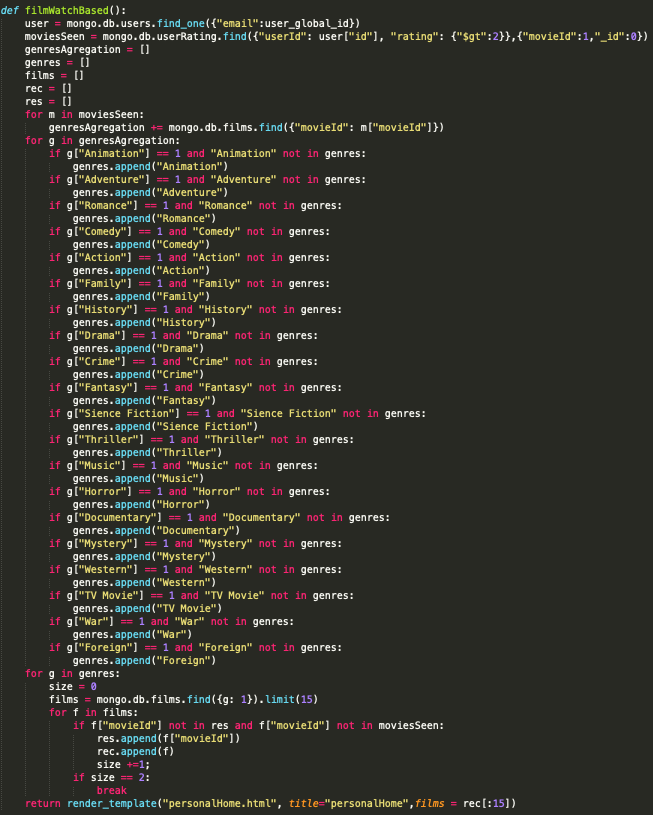
\includegraphics[width=\textwidth]{content.png}
\caption {Função filmWatchBased()}
\label {fig02}
\end{figure}

Este método começa por reunir da coleção userRatings todos os ids dos filmes avaliados de forma positiva pelo utilizador(rating >= 3). De seguida são reunidos os gêneros desse filmes e é feita uma busca na coleção films por esse mesmos géneros. Para cada gênero são colecionados 2 filmes até um máximo de 15 filmes ou até não haver mais gêneros para procurar.


\subsection{Sistemas baseados em conhecimento}


Uma das vantagens destes sistemas é que são particularmente úteis em casos em que não há histórico de filmes ou avaliações, ou cenários de \textit{cold-start}.

\subsubsection{Sistemas baseado em restrições}

Neste caso através de uma search bar o utilizador pode fazer uma pesquisa com uma determinada palavra, frase ou expressão que pode pertencer ao título, ao resumo ou até ao género do filme, e são-lhe apresentados filmes que sejam encontrados nessa busca.
O método encarregue desta busca chama-se \textit{search()}, de seguida apresenta-se o método e explica-se o seu funcionamento.

\begin{figure}[H]
\centering
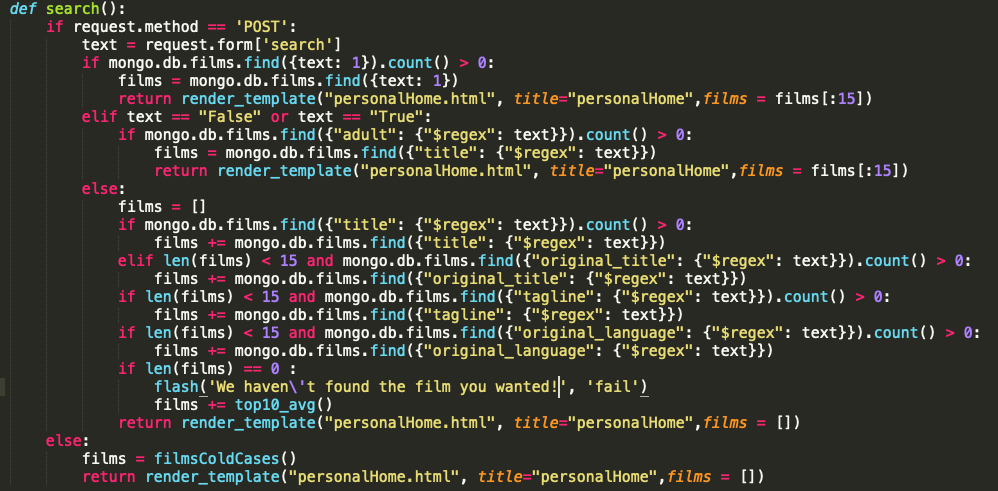
\includegraphics[width=\textwidth]{restricao.png}
\caption {Função search()}
\label {fig03}
\end{figure}
 
Este método começa por verificar se foi chamado por um método \textit{POST} se não foi retorna o método \textit{filmsColdCases()} descrito na próxima subsecção. Caso tal não ocorra este verificará se se trata de um gênero e se se tratar retorna os primeiros 15 filmes escontrados por ele, caso não se trate verifica se a palavra inserida foi "True" ou "False", caso tenha sido realiza uma busca única para verificar se se trata de um filme adulto ou não. Se nenhuma das opções acima descritas foi seguida passamos para uma busca por titulo ou título original, por tagline, por linguagem original e por fim caso não tenhamos resultados suficientes (filmes encontrados == 0), realizamos uma busca pelos 10 melhores filmes e imprimimos uma mensagem a dizer que não encontramos os resultados pretendidos e apresentamos alternativas. 


\subsection{Extras}

Esta subsecção serve para apresentar alguns métodos úteis disponibilizados para melhorar a experiência dos utilizador ou o desempenho da aplicação. 

\subsubsection{Top 10}

\par Caso o utilizador queira ver filmes dos quais provavelmente irá gostar, pode utilizar o método \textit{top10\_avg()} este método é responsável por retornar os 10 filmes mais bem cotados pelo IMDB. Este método foi criado com o objetivo de poder ser uma forma de recomendar bons filmes dos quais o utilizador possa gostar mitigando as dificuldades do cold-start.

\begin{figure}[H]
\centering
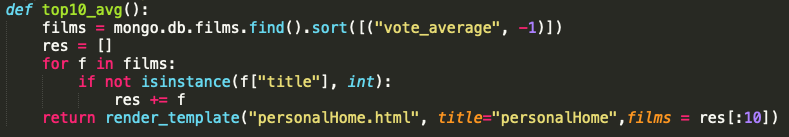
\includegraphics[width=\textwidth]{coldstart.png}
\caption {Função top10\_avg()}
\label {fig04}
\end{figure}

\subsubsection{New Films}

\par Caso tenhamos um filme novo no sistema não dispomos de muitas formas de o promover, o método \textit{filmsColdCases()} resolve esse problema. Primeiro coleciona os filmes por ordem crescente do número de votos, caso tenham o mesmo número de votos ordena-os por data de lançamento. De seguida retira os primeiros 15 documentos obtidos (cada documento corresponde a um filme) e para cada um aumenta em 1 o número de votos na base de dados, isto permite alterar os filmes apresentados visto que eles são ordenados pelo número de votos que possuem, ou seja o seu número de votos vai aumentando sempre, fazendo com que se por exemplo o documento 16 tivesse 0 votos na próxima vez que o método fosse executado este pasaria a ser o primeiro resultado  dado que os 15 anteriores agora teriam 1 voto.

\begin{figure}[H]
\centering
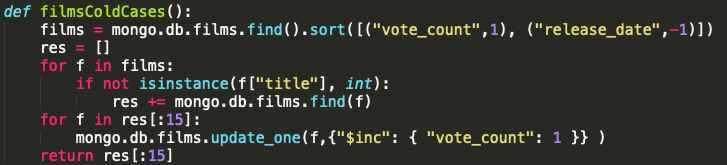
\includegraphics[width=\textwidth]{coldStartFilms.png}
\caption {Função filmsColdCases()}
\label {fig05}
\end{figure}

\subsubsection{Best Rated Films by Users}

\par Se o utilizador quiser ver o que outros utilizadores acham interessante, pode faze-lo graças ao método \textit{memBased()}, este método é útil em situações em que por exemplo o utilizador nunca tenha visto filmes de Drama na plataforma embora goste deles, desta forma caso outros utilizadores tenham visto e dado boa pontuação a filmes deste genero o utilizador pode obter uma excelente recomendação e ao ver esse filme cria uma ponte de ligação entre os seus gostos e os dos utilizadores usados para a recomendação.

\begin{figure}[H]
\centering
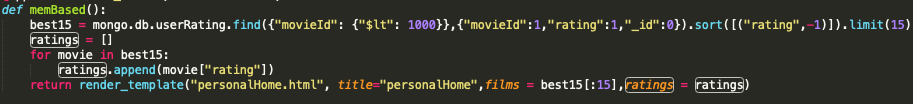
\includegraphics[width=\textwidth]{usersBestRated.png}
\caption {Função memBased()}
\label {fig06}
\end{figure}


\newpage

